\documentclass[12pt, titlepage]{article}

\usepackage{amsmath, mathtools}

\usepackage[round]{natbib}
\usepackage{amsfonts}
\usepackage{amssymb}
\usepackage{graphicx}
\usepackage{colortbl}
\usepackage{xr}
\usepackage{hyperref}
\usepackage{longtable}
\usepackage{xfrac}
\usepackage{tabularx}
\usepackage{float}
\usepackage{siunitx}
\usepackage{booktabs}
\usepackage{multirow}
\usepackage[section]{placeins}
\usepackage{caption}
\usepackage{fullpage}

\hypersetup{
bookmarks=true,     % show bookmarks bar?
colorlinks=true,       % false: boxed links; true: colored links
linkcolor=red,          % color of internal links (change box color with linkbordercolor)
citecolor=blue,      % color of links to bibliography
filecolor=magenta,  % color of file links
urlcolor=cyan          % color of external links
}

\usepackage{array}

%% Comments

\usepackage{color}

\newif\ifcomments\commentstrue %displays comments
%\newif\ifcomments\commentsfalse %so that comments do not display

\ifcomments
\newcommand{\authornote}[3]{\textcolor{#1}{[#3 ---#2]}}
\newcommand{\todo}[1]{\textcolor{red}{[TODO: #1]}}
\else
\newcommand{\authornote}[3]{}
\newcommand{\todo}[1]{}
\fi

\newcommand{\wss}[1]{\authornote{blue}{SS}{#1}} 
\newcommand{\plt}[1]{\authornote{magenta}{TPLT}{#1}} %For explanation of the template
\newcommand{\an}[1]{\authornote{cyan}{Author}{#1}}

%% Common Parts

\newcommand{\progname}{Housemates} % PUT YOUR PROGRAM NAME HERE
\newcommand{\authname}{Team \#9, Housemates
\\ Justin Dang - dangj15 
\\ Harris Hamid - hamidh1
\\ Fady Morcos - morcof2 
\\ Rizwan Ahsan - ahsanm7
\\ Sheikh Afsar - afsars} % AUTHOR NAMES                  

\usepackage{hyperref}
    \hypersetup{colorlinks=true, linkcolor=blue, citecolor=blue, filecolor=blue,
                urlcolor=blue, unicode=false}
    \urlstyle{same}
                                


\begin{document}

\title{Module Interface Specification for \progname{}}

\author{\authname}

\date{\today}

\maketitle

\pagenumbering{roman}

\section{Revision History}

\begin{tabularx}{\textwidth}{p{3cm}p{2cm}X}
\toprule {\bf Date} & {\bf Version} & {\bf Notes}\\
\midrule
January 17, 2024 & 1.0 & Revision 0\\
April 03, 2024 & 2.0 & Revision 1\\
\bottomrule
\end{tabularx}

~\newpage

% \section{Symbols, Abbreviations and Acronyms}

% See SRS Documentation at \wss{give url}

% \wss{Also add any additional symbols, abbreviations or acronyms}

% \newpage

\tableofcontents

\newpage

\pagenumbering{arabic}

\section{Introduction}

The following document details the Module Interface Specifications for \progname{}. The \progname{} app will allow for its users to better communicate with their housemates.  Additionally the app will have a cost management and chore management system to allow for splitting of chores/costs amongst housemates. \\
% \wss{Fill in your project name and description}

Complementary documents include the System Requirement Specifications
and Module Guide.  The full documentation and implementation can be
found at \url{https://github.com/DangJustin/CapstoneProject}.  
% \wss{provide the url for your repo}

\section{Notation}

% \wss{You should describe your notation.  You can use what is below as
%   a starting point.}

The structure of the MIS for modules comes from \citet{HoffmanAndStrooper1995},
with the addition that template modules have been adapted from
\cite{GhezziEtAl2003}.  The mathematical notation comes from Chapter 3 of
\citet{HoffmanAndStrooper1995}.  For instance, the symbol := is used for a
multiple assignment statement and conditional rules follow the form $(c_1
\Rightarrow r_1 | c_2 \Rightarrow r_2 | ... | c_n \Rightarrow r_n )$.

The following table summarizes the primitive data types used by \progname. 

\begin{center}
\renewcommand{\arraystretch}{1.2}
\noindent 
\begin{tabular}{l l p{7.5cm}} 
\toprule 
\textbf{Data Type} & \textbf{Notation} & \textbf{Description}\\ 
\midrule
character & char & a single symbol or digit\\
integer & $\mathbb{Z}$ & a number without a fractional component in (-$\infty$, $\infty$) \\
natural number & $\mathbb{N}$ & a number without a fractional component in [1, $\infty$) \\
real & $\mathbb{R}$ & any number in (-$\infty$, $\infty$)\\
boolean & $\mathbb{B}$ & a boolean value (True or False) \\
\bottomrule
\end{tabular} 
\end{center}

\noindent
The specification of \progname \ uses some derived data types: sequences, strings, and
tuples. Sequences are lists filled with elements of the same data type. Strings
are sequences of characters. Tuples contain a list of values, potentially of
different types. In addition, \progname \ uses functions, which
are defined by the data types of their inputs and outputs. Local functions are
described by giving their type signature followed by their specification.

\section{Module Decomposition}

The following table is taken directly from the Module Guide document for this project.

\begin{table}[h!]
\centering
\begin{tabular}{p{0.3\textwidth} p{0.6\textwidth}}
\toprule
\textbf{Level 1} & \textbf{Level 2}\\
\midrule

{Hardware-Hiding Module} & ~ \\
\midrule

\multirow{7}{0.3\textwidth}{Behaviour-Hiding Module} 
& Task Management Module\\
& Bill Management Module\\
& Scheduling Module\\
& Account Module\\
& Interface Design Module\\
\midrule

\multirow{3}{0.3\textwidth}{Software Decision Module}
& Cryptography Module\\
& Database Interface Module\\
& Network Interface Module\\
\bottomrule

\end{tabular}
\caption{Module Hierarchy}
\label{TblMH}
\end{table}

\newpage
~\newpage


\section{MIS of Task Management Module} \label{mT} 
% \wss{Use labels for cross-referencing}

% \wss{You can reference SRS labels, such as R\ref{R_Inputs}.}

% \wss{It is also possible to use \LaTeX for hypperlinks to external documents.}

\subsection{Module}

TaskManagement

% \wss{Short name for the module}

\subsection{Uses}

Account, InterfaceDesign, DatabaseInterface

\subsection{Syntax}

\subsubsection{Exported Constants}

None

\subsubsection{Exported Access Programs}

\begin{center}
\begin{tabular}{p{3cm} p{5cm} p{2cm} p{4.5cm}}
\hline
\textbf{Name} & \textbf{In} & \textbf{Out} & \textbf{Exceptions} \\
\hline
addTask & taskName: string, groupID: string, deadlineDate: Date, description: string, usersResponsible: seq of string  & seq of string & TaskAddError \\
\hline
getTask & taskID: string & seq of string  & NotFoundError \\
\hline
getUserTasks & userID: string & seq of string  & NotFoundError \\
\hline
completeTask & taskID: string & -  &  NotFoundError \\
\hline
reopenTask & taskID: string & - & NotFoundError \\
\hline
editTask & taskData: seq of string & - & NotFoundError \\
\hline
\end{tabular}
\end{center}

\subsection{Semantics}

\subsubsection{State Variables}

None


% \wss{Not all modules will have state variables.  State variables give the module
%   a memory.}

\subsubsection{Environment Variables}

None

% \wss{This section is not necessary for all modules.  Its purpose is to capture
%   when the module has external interaction with the environment, such as for a
%   device driver, screen interface, keyboard, file, etc.}

\subsubsection{Assumptions}

All taskIDs and userIDs are unique.

% \wss{Try to minimize assumptions and anticipate programmer errors via
%   exceptions, but for practical purposes assumptions are sometimes appropriate.}

\subsubsection{Access Routine Semantics}

\noindent addTask(taskName, groupID, deadlineDate, description, usersResponsible):
\begin{itemize}
\item transition: input data == valid $\Rightarrow$ add task to database
\item output: out := new task returned by database
\item exception:  exc := (invalid input $\vert\vert$ database error $\Rightarrow$ TaskAddError)
\end{itemize}

\noindent getTask(taskID):
\begin{itemize}
\item output: out := task data from taskID
\item exception: exc := (taskID $\notin$ database $\Rightarrow$ NotFoundError)
\end{itemize}

\noindent getUserTasks(userID):
\begin{itemize}
\item output: out := taskIDs of tasks associated with the current userID
\item exception: exc := (userID $\notin$ database $\Rightarrow$ NotFoundError)
\end{itemize}

\noindent completeTask(taskID):
\begin{itemize}
\item transition: taskID $\in$ database $\Rightarrow$ remove from active tasks
\item exception: exc := (taskID $\notin$ database $\Rightarrow$ NotFoundError)
\end{itemize}

\noindent reopenTask(taskID):
\begin{itemize}
\item transition: taskID $\in$ database $\Rightarrow$ add to active tasks
\item exception: exc := (taskID $\notin$ database $\Rightarrow$ NotFoundError)
\end{itemize}

\noindent editTask(taskData):
\begin{itemize}
\item transition: Edit the details of the task
\item exception: exc := (taskID $\notin$ database $\Rightarrow$ NotFoundError)
\end{itemize}


% \wss{A module without environment variables or state variables is unlikely to
%   have a state transition.  In this case a state transition can only occur if
%   the module is changing the state of another module.}

% \wss{Modules rarely have both a transition and an output.  In most cases you
%   will have one or the other.}

\subsubsection{Local Functions}

% \wss{As appropriate} \wss{These functions are for the purpose of specification.
%   They are not necessarily something that is going to be implemented
%   explicitly.  Even if they are implemented, they are not exported; they only
%   have local scope.}

None



\section{MIS of Bill Management Module} \label{mB} 
% % \wss{Use labels forcross-referencing}

% % \wss{You can reference SRS labels, such as R\ref{R_Inputs}.}

% \wss{It is also possible to use \LaTeX for hypperlinks to external documents.}

\subsection{Module}

BillManagement

% \wss{Short name for the module}

\subsection{Uses}

Account, InterfaceDesign, DatabaseInterface

\subsection{Syntax}

\subsubsection{Exported Constants}

None

\subsubsection{Exported Access Programs}

\begin{center}
\begin{tabular}{p{3cm} p{5cm} p{2cm} p{4cm}}
\hline
\textbf{Name} & \textbf{In} & \textbf{Out} & \textbf{Exceptions} \\
\hline
splitExpense & userID: string, amount: $\mathbb{Z}$, billName: string, participants: seq of string, groupID: string, individualAmounts: seq of $\mathbb{Z}$, category: string & - & BillAddError \\
\hline
deleteExpense & billID: string & - & NotFoundError \\
\hline
getExpenses & userID: string & seq of string & NotFoundError\\
\hline
editBill & billID: string, updatedData: seq of string & - & NotFoundError, ValidationError \\
\hline
\end{tabular}
\end{center}

\subsection{Semantics}

\subsubsection{State Variables}

None

% \wss{Not all modules will have state variables.  State variables give the module
%   a memory.}

\subsubsection{Environment Variables}

None

% \wss{This section is not necessary for all modules.  Its purpose is to capture
%   when the module has external interaction with the environment, such as for a
%   device driver, screen interface, keyboard, file, etc.}

\subsubsection{Assumptions}

All billIDs and userIDs are unique.

% \wss{Try to minimize assumptions and anticipate programmer errors via
%   exceptions, but for practical purposes assumptions are sometimes appropriate.}

\subsubsection{Access Routine Semantics}

\noindent splitExpense(userID, amount, billName, participants, groupID, individualAmounts, category):
\begin{itemize}
\item transition: Once the function validates the input data, bill is added into the database using provided parameters.
\item exception: exc := (invalid input $\vert\vert$ database error $\Rightarrow$ BillAddError)
\end{itemize}

\noindent deleteExpense(billID):
\begin{itemize}
\item transition: Remove appropriate amount from the user's total expense and add/remove amount from associated user's.
\item exception: exc := (billID $\notin$ database $\Rightarrow$ NotFoundError)
\end{itemize}

\noindent getExpenses(userID):
\begin{itemize}
\item output: out := billIDs of bills associated with current userID from account module.
\item exception: exc := (billID $\notin$ database $\Rightarrow$ NotFoundError)
\end{itemize}

\noindent editBill(billID, updatedData):
\begin{itemize}
\item transition: Edit the details of the bill
\item exception: exc := (billID $\notin$ database $\Rightarrow$ NotFoundError $\vert$$\vert$ updatedData == invalid $\Rightarrow$ ValidationError)
\end{itemize}

% \wss{A module without environment variables or state variables is unlikely to
%   have a state transition.  In this case a state transition can only occur if
%   the module is changing the state of another module.}

% \wss{Modules rarely have both a transition and an output.  In most cases you
%   will have one or the other.}

% \wss{As appropriate} \wss{These functions are for the purpose of specification.
%   They are not necessarily something that is going to be implemented
%   explicitly.  Even if they are implemented, they are not exported; they only
%   have local scope.}


\section{MIS of Scheduling Module} \label{mB} 
% % \wss{Use labels forcross-referencing}

% % \wss{You can reference SRS labels, such as R\ref{R_Inputs}.}

% \wss{It is also possible to use \LaTeX for hypperlinks to external documents.}

\subsection{Module}

Scheduling

% \wss{Short name for the module}

\subsection{Uses}

DatabaseInterface, InterfaceDesign, Account

\subsection{Syntax}

\subsubsection{Exported Constants}

None

\subsubsection{Exported Access Programs}

\begin{center}
\begin{tabular}{p{3cm} p{4cm} p{4cm} p{4.5cm}}
\hline
\textbf{Name} & \textbf{In} & \textbf{Out} & \textbf{Exceptions} \\
\hline
addEvent & eventName: string, dateTime: Date, endDateTime: Date, groupID: string & seq of string & EventAddError \\
\hline
editEvent & eventID: string, updateData: seq of string & seq of string & NotFoundError,  ValidationError \\
\hline
deleteEvent & eventID: string & - & NotFoundError\\
\hline
getGroupEvents & groupID: string & seq of string & NotFoundError\\
\hline
getUserEvents & userID: string & seq of string & NotFoundError\\
\hline
\end{tabular}
\end{center}

\subsection{Semantics}

\subsubsection{State Variables}

None

% \wss{Not all modules will have state variables.  State variables give the module
%   a memory.}

\subsubsection{Environment Variables}

None

% \wss{This section is not necessary for all modules.  Its purpose is to capture
%   when the module has external interaction with the environment, such as for a
%   device driver, screen interface, keyboard, file, etc.}

\subsubsection{Assumptions}

All eventIDs, groupIDs and userIDs are unique.

% \wss{Try to minimize assumptions and anticipate programmer errors via
%   exceptions, but for practical purposes assumptions are sometimes appropriate.}

\subsubsection{Access Routine Semantics}

\noindent addEvent(eventName, dateTime, endDateTime, groupID):
\begin{itemize}
\item transition: create event in database using parameter.
\item output: out := eventID returned by database.
\item exception:  exc := (invalid input $\vert\vert$ database error $\Rightarrow$ EventAddError)
\end{itemize}

\noindent editEvent(eventID, updateData):
\begin{itemize}
\item transition: eventID $\in$ database \&\& updateData == valid $\Rightarrow$ update event
\item output: out := event data returned by database.
\item exception: exc := (eventID $\notin$ database $\Rightarrow$ NotFoundError $\vert$$\vert$ updateData == invalid $\Rightarrow$ ValidationError)
\end{itemize}

\noindent deleteEvent(eventID):
\begin{itemize}
\item transition: eventID $\in$ database $\Rightarrow$ delete event
\item exception: exc := (eventID $\notin$ database $\Rightarrow$ NotFoundError)
\end{itemize}

\noindent getGroupEvents(groupID):
\begin{itemize}
\item output: out := details of Events associated with groupID in the database.
\item exception: exc := (groupID $\notin$ database $\Rightarrow$ NotFoundError)
\end{itemize}

\noindent getUserEvents(userID):
\begin{itemize}
\item output: out := details of Events associated with userID in the database.
\item exception: exc := (userID $\notin$ database $\Rightarrow$ NotFoundError)
\end{itemize}

% \wss{A module without environment variables or state variables is unlikely to
%   have a state transition.  In this case a state transition can only occur if
%   the module is changing the state of another module.}

% \wss{Modules rarely have both a transition and an output.  In most cases you
%   will have one or the other.}

\subsubsection{Local Functions}

None

% \wss{As appropriate} \wss{These functions are for the purpose of specification.
%   They are not necessarily something that is going to be implemented
%   explicitly.  Even if they are implemented, they are not exported; they only
%   have local scope.}


\section{MIS of Account Module} \label{mB} 
% % \wss{Use labels forcross-referencing}

% % \wss{You can reference SRS labels, such as R\ref{R_Inputs}.}

% \wss{It is also possible to use \LaTeX for hypperlinks to external documents.}

\subsection{Module}

Account

% \wss{Short name for the module}

\subsection{Uses}

DatabaseInterface, InterfaceDesign

\subsection{Syntax}

\subsubsection{Exported Constants}

None

\subsubsection{Exported Access Programs}

\begin{center}
\begin{tabular}{p{3cm} p{4.5cm} p{4cm} p{4.5cm}}
\hline
\textbf{Name} & \textbf{In} & \textbf{Out} & \textbf{Exceptions} \\
\hline
createAccount & userData: Tuple of (userName: string, password: string, firstName: string, lastName: string, phone: string, email: string) & - & UserCreationError \\
\hline
login & email: string, password: string & string & ValidationError \\
\hline
getUserGroups & userID: string & seq of string  & NotFoundError \\
\hline
getUser & userID: string & seq of string & NotFoundError \\
\hline
getGroup & groupID: string & seq of string & NotFoundError \\
\hline
logout & - & - & - \\
\hline
deleteAccount & email: string, password: string & - & ValidationError \\
\hline
\end{tabular}
\end{center}

\subsection{Semantics}

\subsubsection{State Variables}

None

% \wss{Not all modules will have state variables.  State variables give the module
%   a memory.}

\subsubsection{Environment Variables}

None

% \wss{This section is not necessary for all modules.  Its purpose is to capture
%   when the module has external interaction with the environment, such as for a
%   device driver, screen interface, keyboard, file, etc.}

\subsubsection{Assumptions}

All UserIDs and GroupIDs are unique

% \wss{Try to minimize assumptions and anticipate programmer errors via
%   exceptions, but for practical purposes assumptions are sometimes appropriate.}

\subsubsection{Access Routine Semantics}

\noindent createAccount(userData):
\begin{itemize}
\item transition: create user in database using userData parameter
\item exception:  exc := (invalid input $\vert\vert$ database error $\Rightarrow$ UserCreationError)
\end{itemize}

\noindent login(email, password):
\begin{itemize}
\item transition: email $\in$ database \&\& correct password $\Rightarrow$ login user
\item ouput: out := userID
\item exception: exc := (email $\notin$ database $\vert\vert$ wrong password $\Rightarrow$ ValidationError)
\end{itemize}

\noindent getUserGroups(userID):
\begin{itemize}
\item output: out := (userID $\in$ database $\Rightarrow$ group data)
\item exception: exc := (userID $\notin$ database $\Rightarrow$ NotFoundError)
\end{itemize}

\noindent getUser(userID):
\begin{itemize}
\item output: out := (userID $\in$ database $\Rightarrow$ user data)
\item exception: exc := (userID $\notin$ database $\Rightarrow$ NotFoundError)
\end{itemize}

\noindent getGroup(groupID):
\begin{itemize}
\item output: out := (groupID $\in$ database $\Rightarrow$ group data)
\item exception: exc := (groupID $\notin$ database $\Rightarrow$ NotFoundError)
\end{itemize}

\noindent logout():
\begin{itemize}
\item transition: log out user in database
\item exception: none
\end{itemize}

\noindent deleteAccount(email, password):
\begin{itemize}
\item transition: email $\in$ database \&\& correct password $\Rightarrow$ delete user
\item exception: exc := (email $\notin$ database $\vert\vert$ wrong password $\Rightarrow$ ValidationError)
\end{itemize}

% \wss{A module without environment variables or state variables is unlikely to
%   have a state transition.  In this case a state transition can only occur if
%   the module is changing the state of another module.}

% \wss{Modules rarely have both a transition and an output.  In most cases you
%   will have one or the other.}

\subsubsection{Local Functions}

None

% \wss{As appropriate} \wss{These functions are for the purpose of specification.
%   They are not necessarily something that is going to be implemented
%   explicitly.  Even if they are implemented, they are not exported; they only
%   have local scope.}



% \section{MIS of \wss{Module Name}} \label{Module} \wss{Use labels for
%   cross-referencing}

% \wss{You can reference SRS labels, such as R\ref{R_Inputs}.}

% \wss{It is also possible to use \LaTeX for hypperlinks to external documents.}

% \subsection{Module}

% \wss{Short name for the module}

% \subsection{Uses}

% \subsection{Syntax}

% \subsubsection{Exported Constants}

% \subsubsection{Exported Access Programs}

% \begin{center}
% \begin{tabular}{p{2cm} p{4cm} p{4cm} p{2cm}}
% \hline
% \textbf{Name} & \textbf{In} & \textbf{Out} & \textbf{Exceptions} \\
% \hline
% \wss{accessProg} & - & - & - \\
% \hline
% \end{tabular}
% \end{center}

% \subsection{Semantics}

% \subsubsection{State Variables}

% \wss{Not all modules will have state variables.  State variables give the module
%   a memory.}

% \subsubsection{Environment Variables}

% \wss{This section is not necessary for all modules.  Its purpose is to capture
%   when the module has external interaction with the environment, such as for a
%   device driver, screen interface, keyboard, file, etc.}

% \subsubsection{Assumptions}

% \wss{Try to minimize assumptions and anticipate programmer errors via
%   exceptions, but for practical purposes assumptions are sometimes appropriate.}

% \subsubsection{Access Routine Semantics}

% \noindent \wss{accessProg}():
% \begin{itemize}
% \item transition: \wss{if appropriate} 
% \item output: \wss{if appropriate} 
% \item exception: \wss{if appropriate} 
% \end{itemize}

% \wss{A module without environment variables or state variables is unlikely to
%   have a state transition.  In this case a state transition can only occur if
%   the module is changing the state of another module.}

% \wss{Modules rarely have both a transition and an output.  In most cases you
%   will have one or the other.}

% \subsubsection{Local Functions}

% \wss{As appropriate} \wss{These functions are for the purpose of specification.
%   They are not necessarily something that is going to be implemented
%   explicitly.  Even if they are implemented, they are not exported; they only
%   have local scope.}

\newpage

\bibliographystyle {plainnat}
\bibliography {MIS.bib}

\newpage

\section{Appendix} \label{Appendix}

\subsection{Database Specification} \label{Database}
In this section, the description of the database schema of \progname{} will be provided. The database for \progname{} will be relatively simple with only a few entities (account, user, task, group, events, bills) which cover the main functionalities of \progname{}. The relationships between these entities are described in Figure \ref{FigDB}.

\begin{figure}[H]
\centering
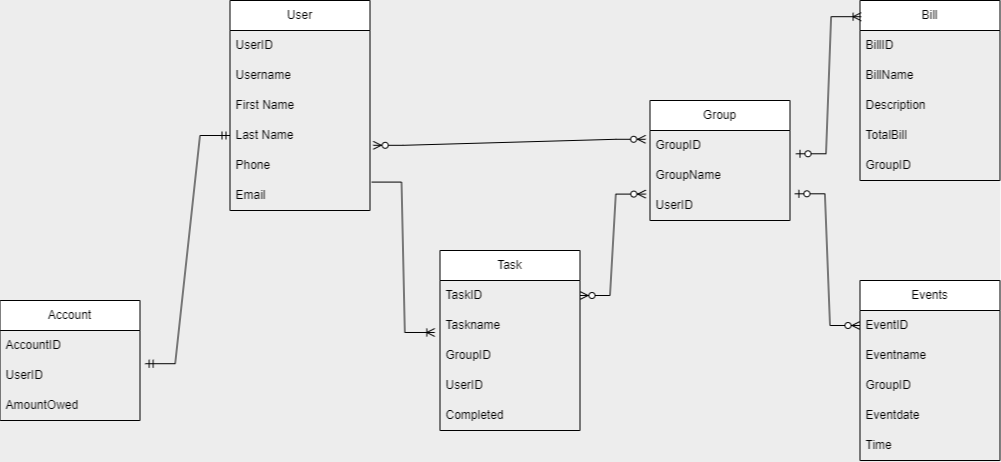
\includegraphics[width=\linewidth]{Database.png}
\caption{Entity-Relationship Diagram of the Housemates Database}
\label{FigDB}
\end{figure}
% Put database relational diagram here

\subsection{Interface Specification} \label{Interface}

In this section, the description of the user interface of \progname{} will be provided. The user interface of \progname{} is designed to be minimalist and simple to use. This will allow the users of \progname{} to quickly access the main functions of \progname{}. Some examples of the interface are described in the figures below and at \url{https://www.figma.com/file/lMZxonql0nhowgpIslIwns/Housemates-Interface-Design?type=design&node-id=0%3A1&mode=design&t=iuU1JQzgxRP93dCL-1}. The interface for \progname{} may change in the final implementation.

\begin{figure}[H]
\centering
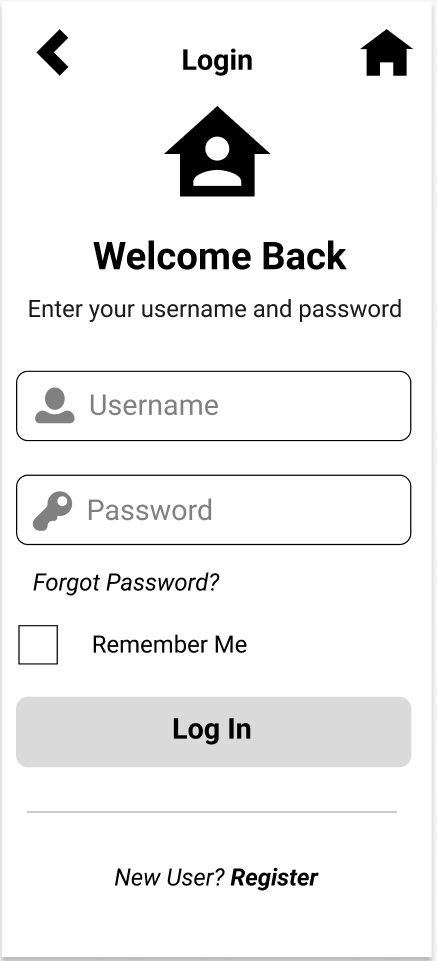
\includegraphics[width=\textwidth]{Login.png}
\caption{Login screen of \progname{}}
\label{FigLogin}
\end{figure}

\begin{figure}[H]
\centering
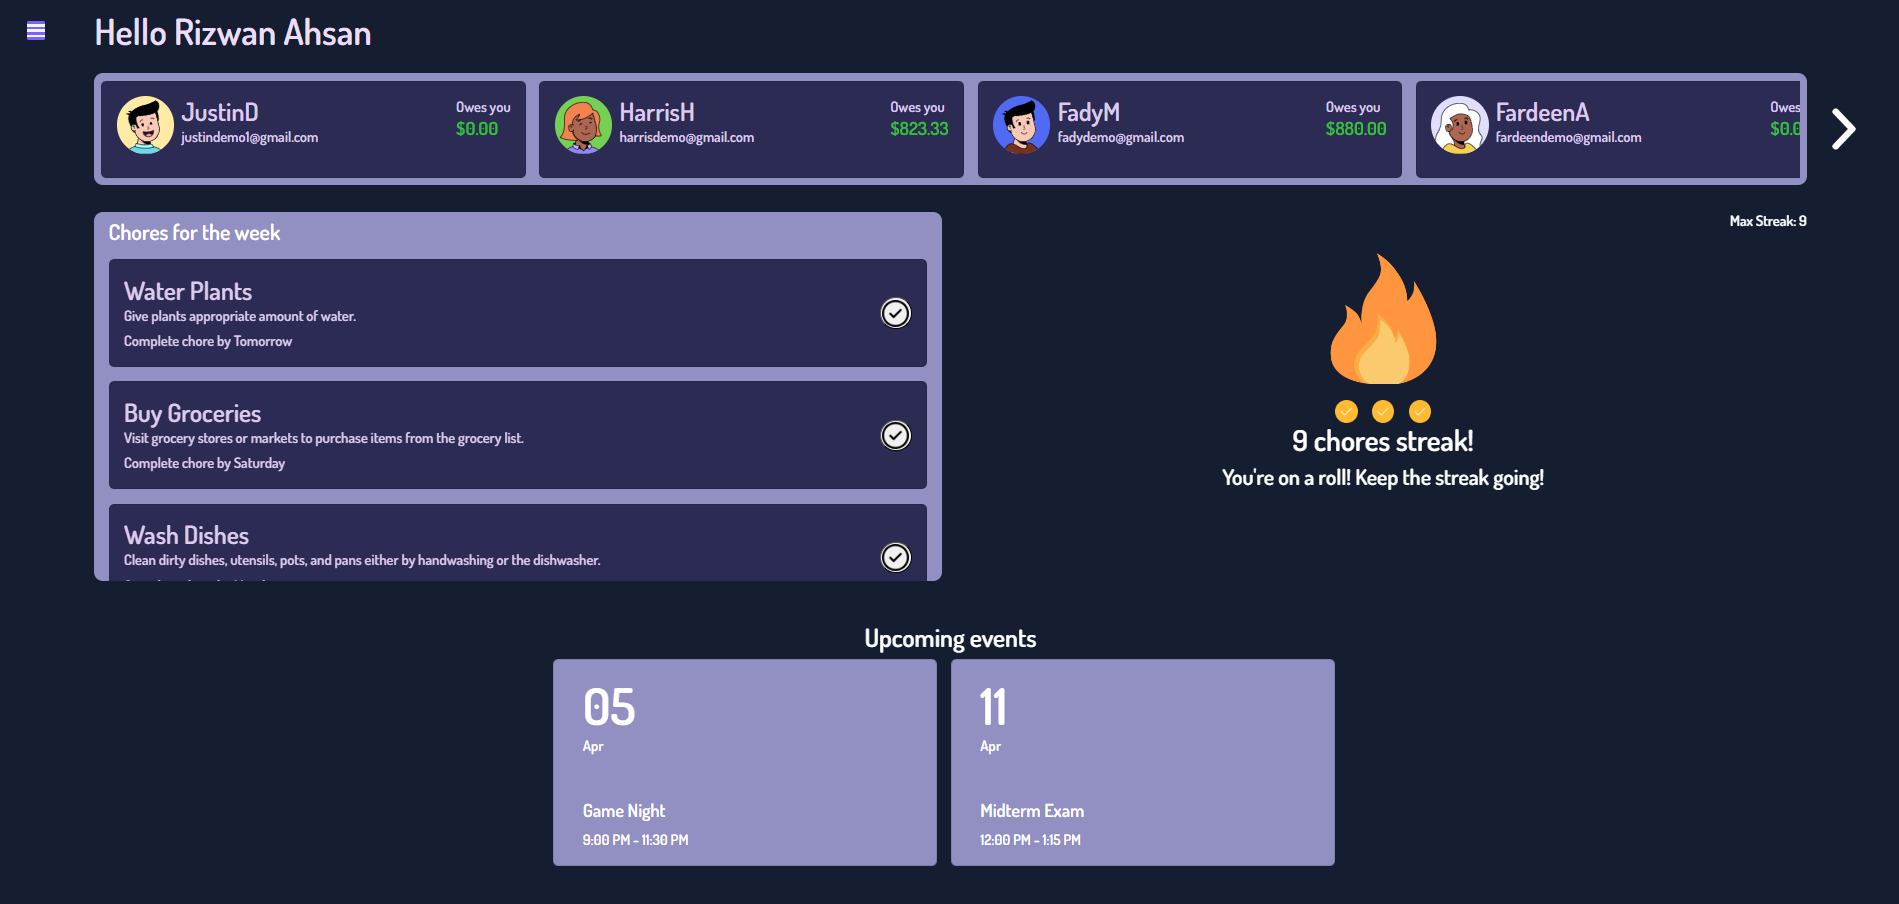
\includegraphics[width=\textwidth]{Homescreen.png}
\caption{Homescreen of \progname{}}
\label{FigHome}
\end{figure}

\begin{figure}[H]
\centering
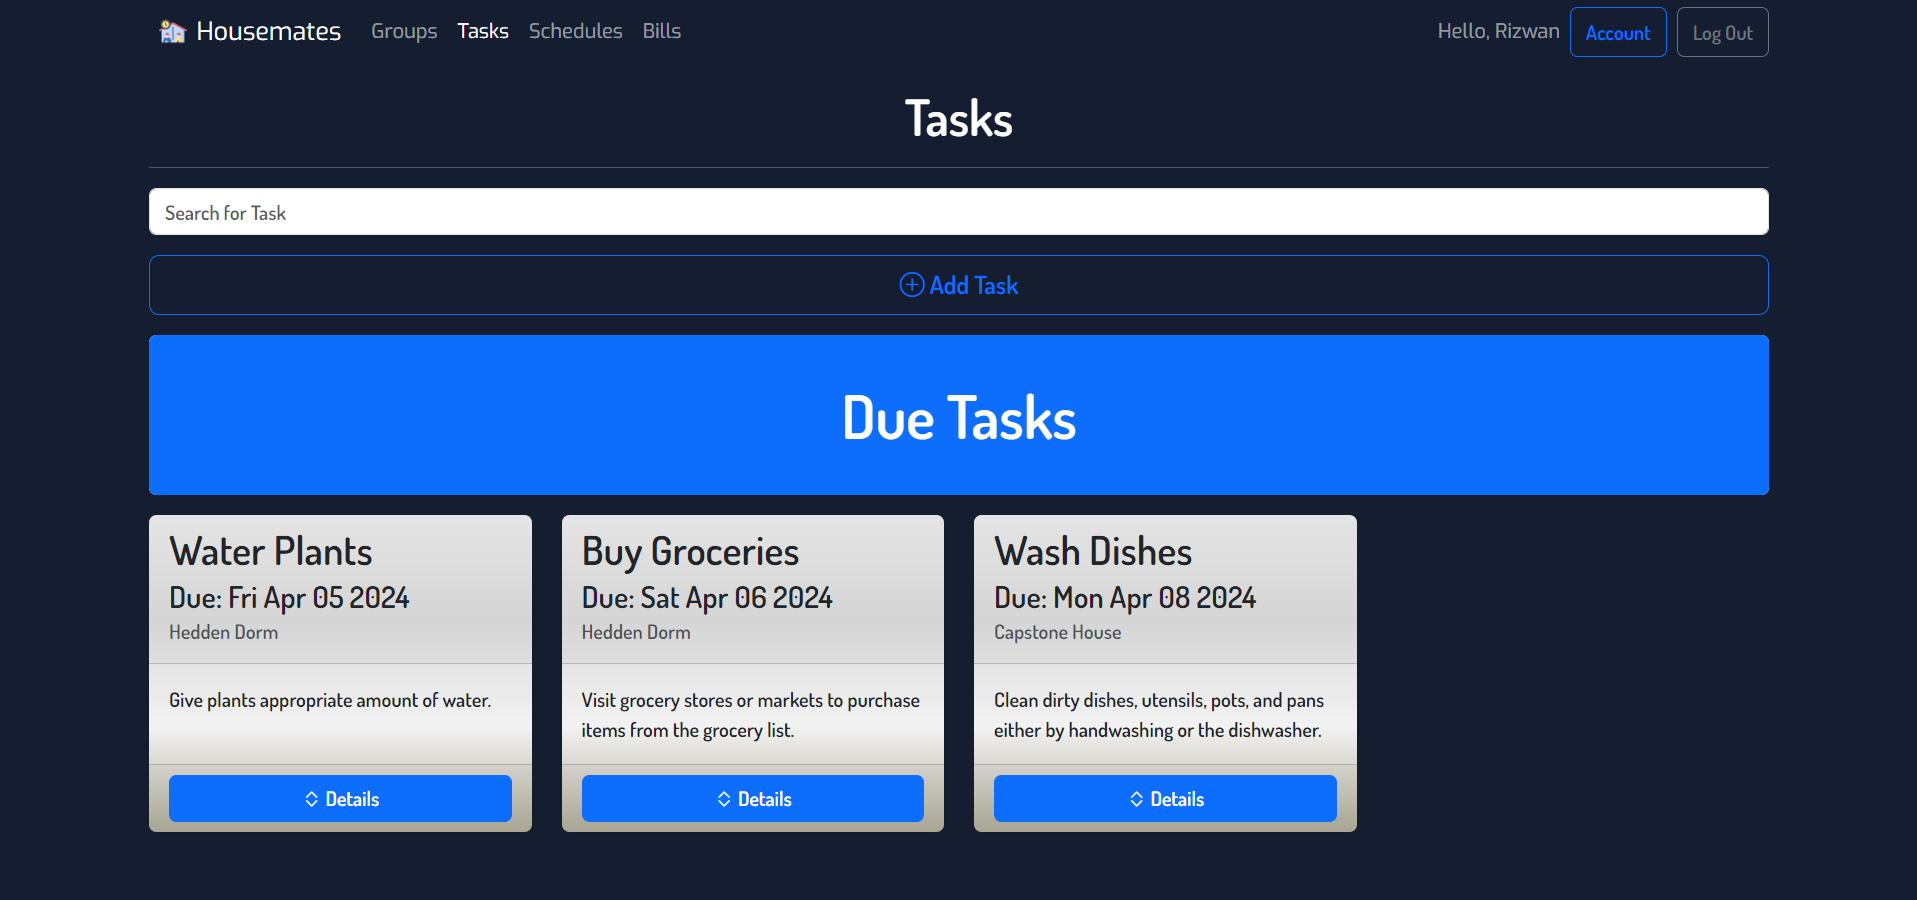
\includegraphics[width=\textwidth]{Task.png}
\caption{Task screen of \progname{}}
\label{FigAccount}
\end{figure}

\begin{figure}[H]
\centering
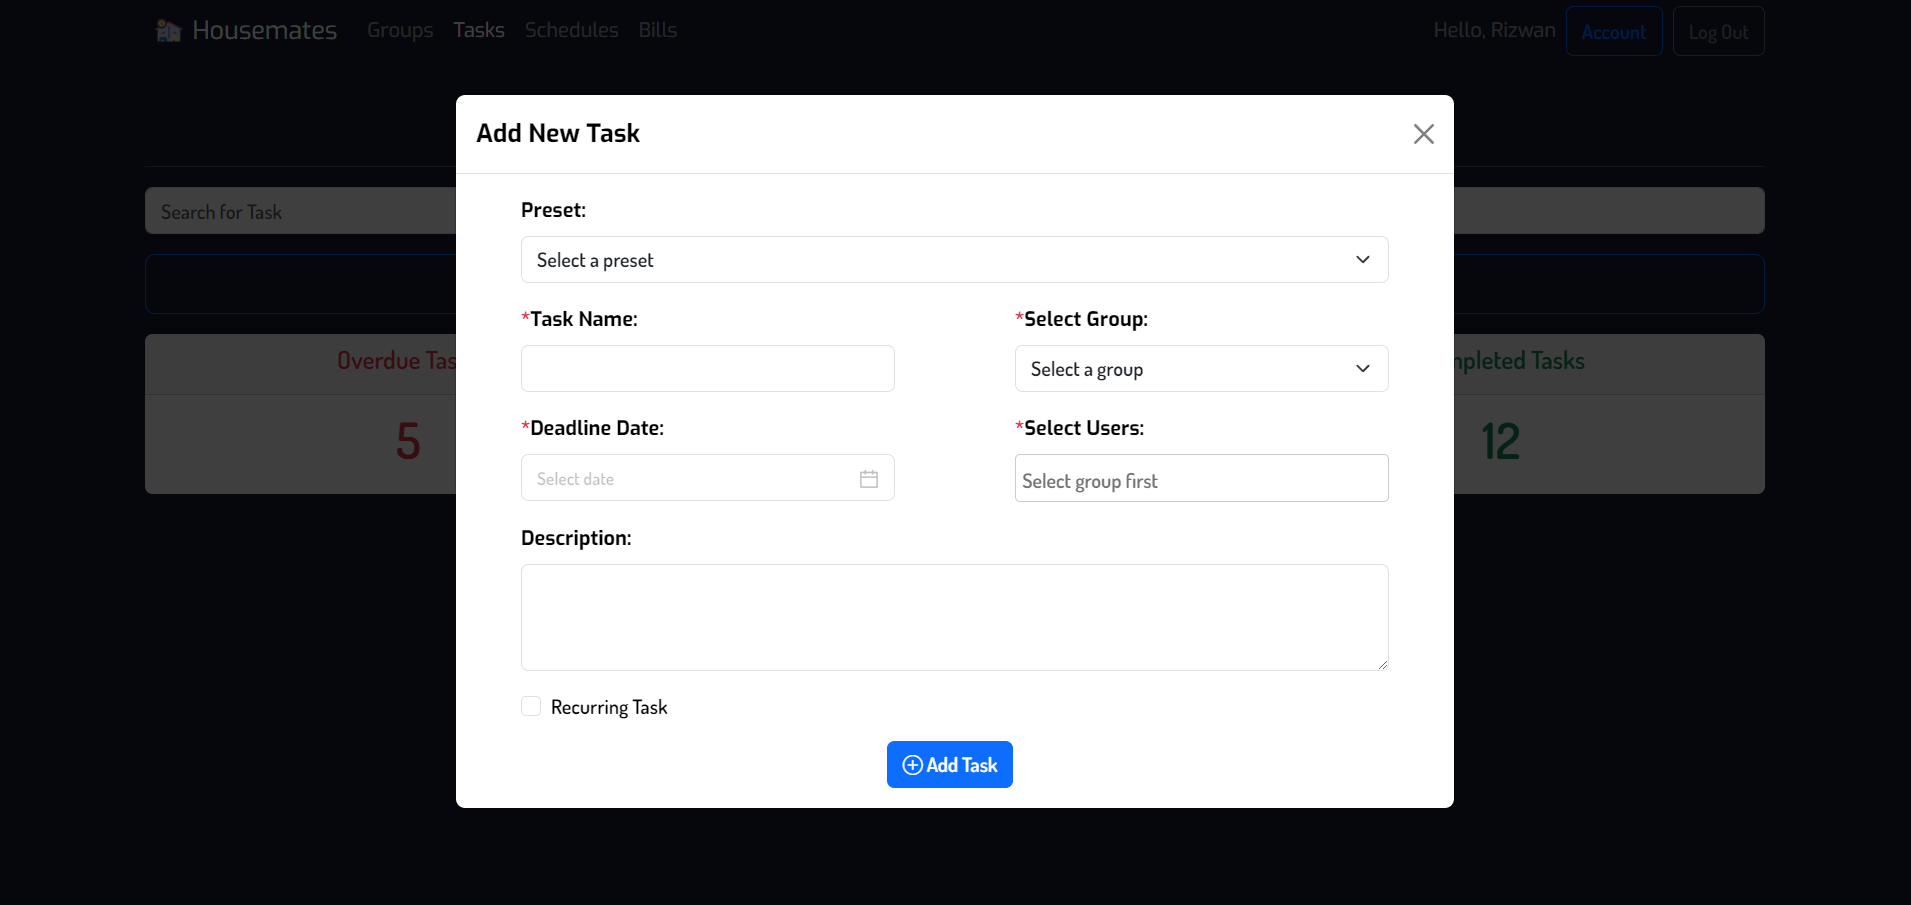
\includegraphics[width=\textwidth]{AddTask.png}
\caption{Add tasks screen of \progname{}}
\label{FigTasks}
\end{figure}

\begin{figure}[H]
\centering
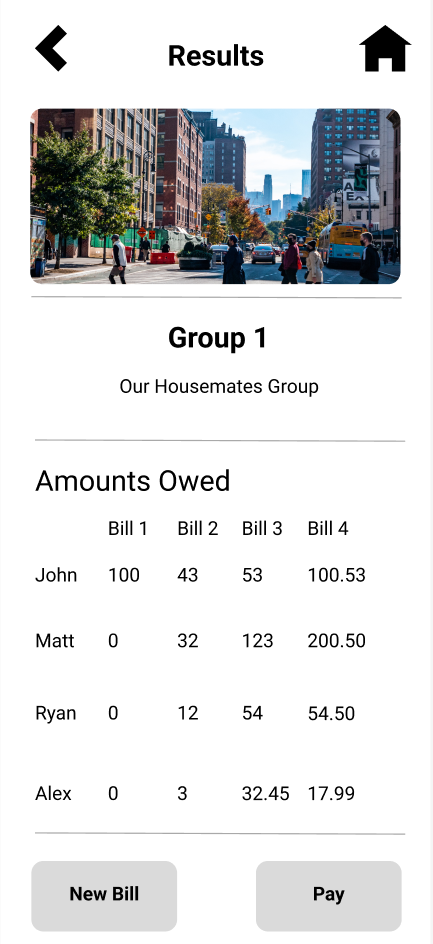
\includegraphics[width=\textwidth]{Bills.png}
\caption{Bills screen of \progname{}}
\label{FigBills}
\end{figure}

\begin{figure}[H]
\centering
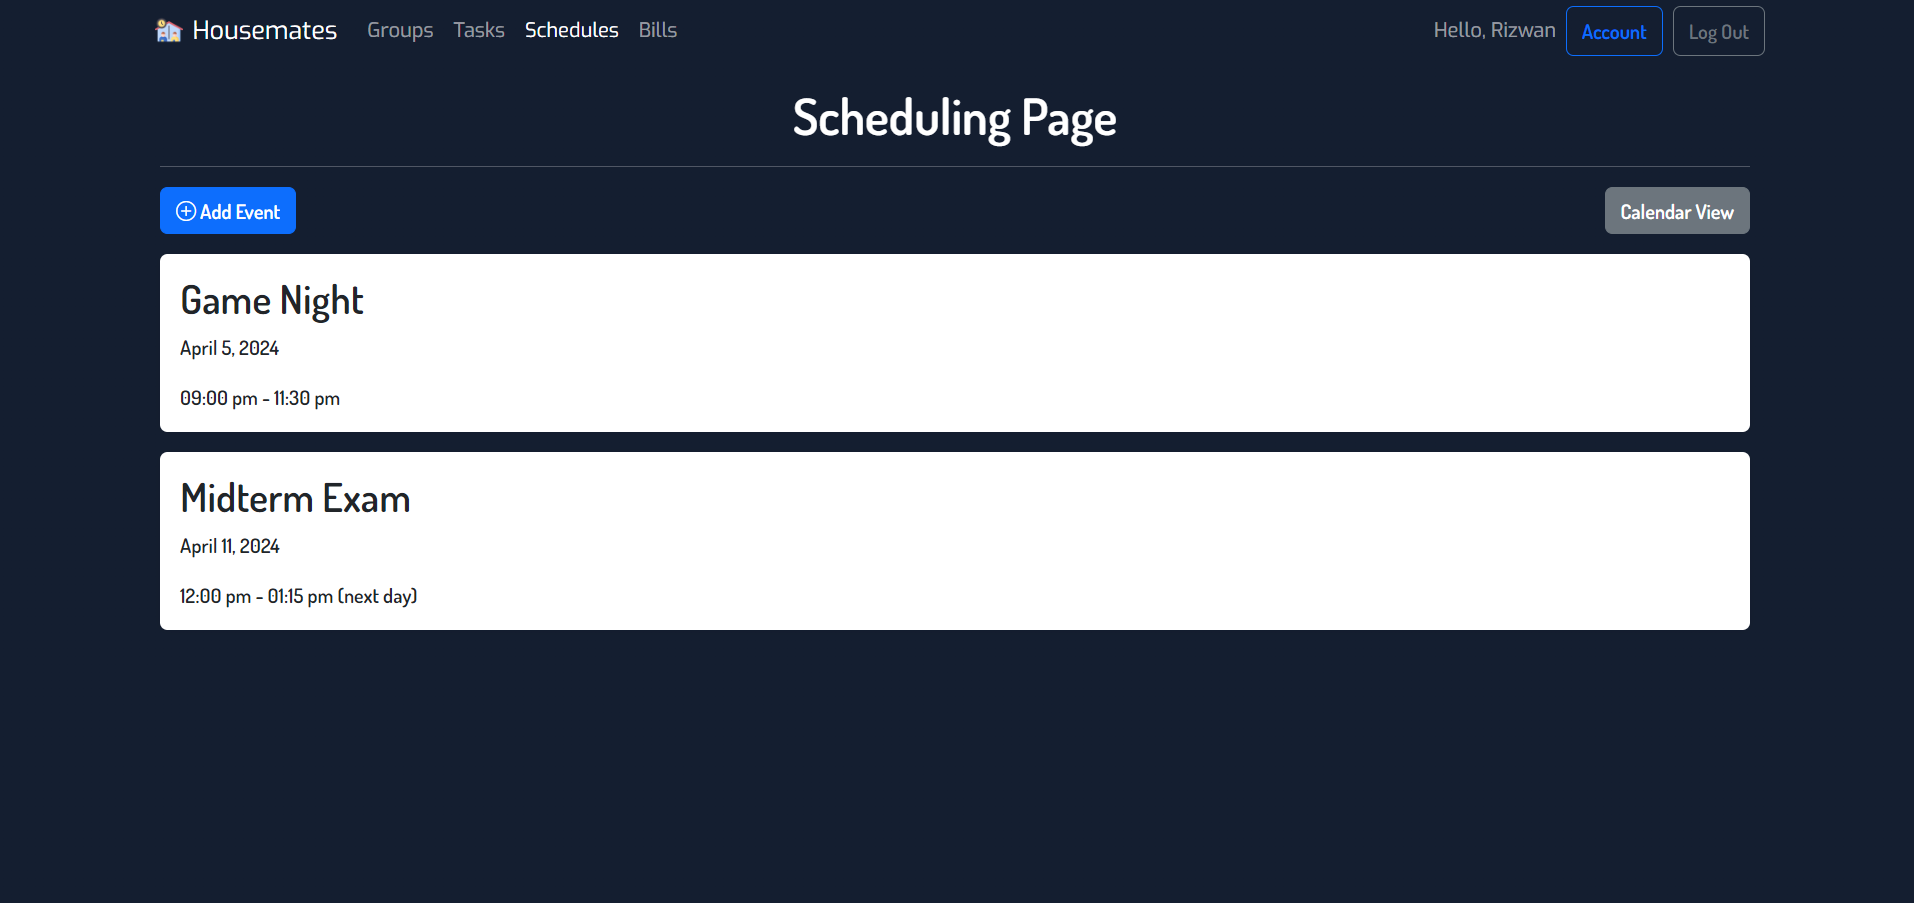
\includegraphics[width=\textwidth]{Events.png}
\caption{Scheduling screen of \progname{}}
\label{FigEvents}
\end{figure}

% \wss{Extra information if required}

\end{document}